\documentclass[1p]{elsarticle_modified}
%\bibliographystyle{elsarticle-num}

%\usepackage[colorlinks]{hyperref}
%\usepackage{abbrmath_seonhwa} %\Abb, \Ascr, \Acal ,\Abf, \Afrak
\usepackage{amsfonts}
\usepackage{amssymb}
\usepackage{amsmath}
\usepackage{amsthm}
\usepackage{scalefnt}
\usepackage{amsbsy}
\usepackage{kotex}
\usepackage{caption}
\usepackage{subfig}
\usepackage{color}
\usepackage{graphicx}
\usepackage{xcolor} %% white, black, red, green, blue, cyan, magenta, yellow
\usepackage{float}
\usepackage{setspace}
\usepackage{hyperref}

\usepackage{tikz}
\usetikzlibrary{arrows}

\usepackage{multirow}
\usepackage{array} % fixed length table
\usepackage{hhline}

%%%%%%%%%%%%%%%%%%%%%
\makeatletter
\renewcommand*\env@matrix[1][\arraystretch]{%
	\edef\arraystretch{#1}%
	\hskip -\arraycolsep
	\let\@ifnextchar\new@ifnextchar
	\array{*\c@MaxMatrixCols c}}
\makeatother %https://tex.stackexchange.com/questions/14071/how-can-i-increase-the-line-spacing-in-a-matrix
%%%%%%%%%%%%%%%

\usepackage[normalem]{ulem}

\newcommand{\msout}[1]{\ifmmode\text{\sout{\ensuremath{#1}}}\else\sout{#1}\fi}
%SOURCE: \msout is \stkout macro in https://tex.stackexchange.com/questions/20609/strikeout-in-math-mode

\newcommand{\cancel}[1]{
	\ifmmode
	{\color{red}\msout{#1}}
	\else
	{\color{red}\sout{#1}}
	\fi
}

\newcommand{\add}[1]{
	{\color{blue}\uwave{#1}}
}

\newcommand{\replace}[2]{
	\ifmmode
	{\color{red}\msout{#1}}{\color{blue}\uwave{#2}}
	\else
	{\color{red}\sout{#1}}{\color{blue}\uwave{#2}}
	\fi
}

\newcommand{\Sol}{\mathcal{S}} %segment
\newcommand{\D}{D} %diagram
\newcommand{\A}{\mathcal{A}} %arc


%%%%%%%%%%%%%%%%%%%%%%%%%%%%%5 test

\def\sl{\operatorname{\textup{SL}}(2,\Cbb)}
\def\psl{\operatorname{\textup{PSL}}(2,\Cbb)}
\def\quan{\mkern 1mu \triangleright \mkern 1mu}

\theoremstyle{definition}
\newtheorem{thm}{Theorem}[section]
\newtheorem{prop}[thm]{Proposition}
\newtheorem{lem}[thm]{Lemma}
\newtheorem{ques}[thm]{Question}
\newtheorem{cor}[thm]{Corollary}
\newtheorem{defn}[thm]{Definition}
\newtheorem{exam}[thm]{Example}
\newtheorem{rmk}[thm]{Remark}
\newtheorem{alg}[thm]{Algorithm}

\newcommand{\I}{\sqrt{-1}}
\begin{document}

%\begin{frontmatter}
%
%\title{Boundary parabolic representations of knots up to 8 crossings}
%
%%% Group authors per affiliation:
%\author{Yunhi Cho} 
%\address{Department of Mathematics, University of Seoul, Seoul, Korea}
%\ead{yhcho@uos.ac.kr}
%
%
%\author{Seonhwa Kim} %\fnref{s_kim}}
%\address{Center for Geometry and Physics, Institute for Basic Science, Pohang, 37673, Korea}
%\ead{ryeona17@ibs.re.kr}
%
%\author{Hyuk Kim}
%\address{Department of Mathematical Sciences, Seoul National University, Seoul 08826, Korea}
%\ead{hyukkim@snu.ac.kr}
%
%\author{Seokbeom Yoon}
%\address{Department of Mathematical Sciences, Seoul National University, Seoul, 08826,  Korea}
%\ead{sbyoon15@snu.ac.kr}
%
%\begin{abstract}
%We find all boundary parabolic representation of knots up to 8 crossings.
%
%\end{abstract}
%\begin{keyword}
%    \MSC[2010] 57M25 
%\end{keyword}
%
%\end{frontmatter}

%\linenumbers
%\tableofcontents
%
\newcommand\colored[1]{\textcolor{white}{\rule[-0.35ex]{0.8em}{1.4ex}}\kern-0.8em\color{red} #1}%
%\newcommand\colored[1]{\textcolor{white}{ #1}\kern-2.17ex	\textcolor{white}{ #1}\kern-1.81ex	\textcolor{white}{ #1}\kern-2.15ex\color{red}#1	}

{\Large $\underline{11n_{135}~(K11n_{135})}$}

\setlength{\tabcolsep}{10pt}
\renewcommand{\arraystretch}{1.6}
\vspace{1cm}\begin{tabular}{m{100pt}>{\centering\arraybackslash}m{274pt}}
\multirow{5}{120pt}{
	\centering
	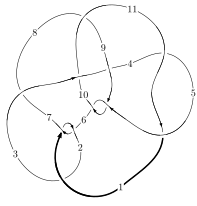
\includegraphics[width=112pt]{../../../GIT/diagram.site/Diagrams/png/751_11n_135.png}\\
\ \ \ A knot diagram\footnotemark}&
\allowdisplaybreaks
\textbf{Linearized knot diagam} \\
\cline{2-2}
 &
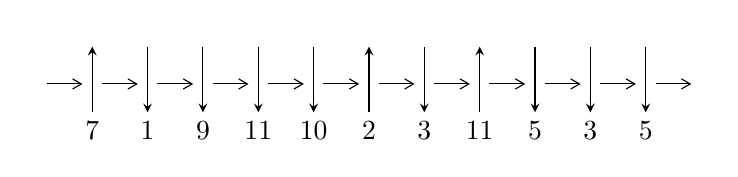
\begin{tikzpicture}[x=20pt, y=17pt]
	% nodes
	\node (C0) at (0, 0) {};
	\node (C1) at (1, 0) {};
	\node (C1U) at (1, +1) {};
	\node (C1D) at (1, -1) {7};

	\node (C2) at (2, 0) {};
	\node (C2U) at (2, +1) {};
	\node (C2D) at (2, -1) {1};

	\node (C3) at (3, 0) {};
	\node (C3U) at (3, +1) {};
	\node (C3D) at (3, -1) {9};

	\node (C4) at (4, 0) {};
	\node (C4U) at (4, +1) {};
	\node (C4D) at (4, -1) {11};

	\node (C5) at (5, 0) {};
	\node (C5U) at (5, +1) {};
	\node (C5D) at (5, -1) {10};

	\node (C6) at (6, 0) {};
	\node (C6U) at (6, +1) {};
	\node (C6D) at (6, -1) {2};

	\node (C7) at (7, 0) {};
	\node (C7U) at (7, +1) {};
	\node (C7D) at (7, -1) {3};

	\node (C8) at (8, 0) {};
	\node (C8U) at (8, +1) {};
	\node (C8D) at (8, -1) {11};

	\node (C9) at (9, 0) {};
	\node (C9U) at (9, +1) {};
	\node (C9D) at (9, -1) {5};

	\node (C10) at (10, 0) {};
	\node (C10U) at (10, +1) {};
	\node (C10D) at (10, -1) {3};

	\node (C11) at (11, 0) {};
	\node (C11U) at (11, +1) {};
	\node (C11D) at (11, -1) {5};
	\node (C12) at (12, 0) {};

	% arrows
	\draw[->,>={angle 60}]
	(C0) edge (C1) (C1) edge (C2) (C2) edge (C3) (C3) edge (C4) (C4) edge (C5) (C5) edge (C6) (C6) edge (C7) (C7) edge (C8) (C8) edge (C9) (C9) edge (C10) (C10) edge (C11) (C11) edge (C12) ;	\draw[->,>=stealth]
	(C1D) edge (C1U) (C2U) edge (C2D) (C3U) edge (C3D) (C4U) edge (C4D) (C5U) edge (C5D) (C6D) edge (C6U) (C7U) edge (C7D) (C8D) edge (C8U) (C9U) edge (C9D) (C10U) edge (C10D) (C11U) edge (C11D) ;
	\end{tikzpicture} \\
\hhline{~~} \\& 
\textbf{Solving Sequence} \\ \cline{2-2} 
 &
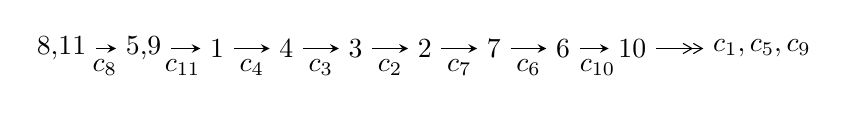
\begin{tikzpicture}[x=25pt, y=7pt]
	% node
	\node (A0) at (-1/8, 0) {8,11};
	\node (A1) at (17/16, 0) {5,9};
	\node (A2) at (17/8, 0) {1};
	\node (A3) at (25/8, 0) {4};
	\node (A4) at (33/8, 0) {3};
	\node (A5) at (41/8, 0) {2};
	\node (A6) at (49/8, 0) {7};
	\node (A7) at (57/8, 0) {6};
	\node (A8) at (65/8, 0) {10};
	\node (C1) at (1/2, -1) {$c_{8}$};
	\node (C2) at (13/8, -1) {$c_{11}$};
	\node (C3) at (21/8, -1) {$c_{4}$};
	\node (C4) at (29/8, -1) {$c_{3}$};
	\node (C5) at (37/8, -1) {$c_{2}$};
	\node (C6) at (45/8, -1) {$c_{7}$};
	\node (C7) at (53/8, -1) {$c_{6}$};
	\node (C8) at (61/8, -1) {$c_{10}$};
	\node (A9) at (10, 0) {$c_{1},c_{5},c_{9}$};

	% edge
	\draw[->,>=stealth]	
	(A0) edge (A1) (A1) edge (A2) (A2) edge (A3) (A3) edge (A4) (A4) edge (A5) (A5) edge (A6) (A6) edge (A7) (A7) edge (A8) ;
	\draw[->>,>={angle 60}]	
	(A8) edge (A9);
\end{tikzpicture} \\ 

\end{tabular} \\

\footnotetext{
The image of knot diagram is generated by the software ``\textbf{Draw programme}" developed by Andrew Bartholomew(\url{http://www.layer8.co.uk/maths/draw/index.htm\#Running-draw}), where we modified some parts for our purpose(\url{https://github.com/CATsTAILs/LinksPainter}).
}\phantom \\ \newline 
\centering \textbf{Ideals for irreducible components\footnotemark of $X_{\text{par}}$} 
 
\begin{align*}
I^u_{1}&=\langle 
7 u^9-24 u^8-34 u^7+183 u^6-48 u^5-359 u^4+366 u^3-130 u^2+b+40 u-13,\\
\phantom{I^u_{1}}&\phantom{= \langle  }-13 u^9+45 u^8+63 u^7-343 u^6+90 u^5+672 u^4-681 u^3+245 u^2+a-78 u+25,\\
\phantom{I^u_{1}}&\phantom{= \langle  }u^{10}-4 u^9-3 u^8+29 u^7-21 u^6-48 u^5+80 u^4-47 u^3+16 u^2-5 u+1\rangle \\
I^u_{2}&=\langle 
-2 u^7-11 u^6-18 u^5-6 u^4+u^3-5 u^2+b- u-2,\;2 u^7+12 u^6+23 u^5+12 u^4-4 u^3+u^2+a+5 u+3,\\
\phantom{I^u_{2}}&\phantom{= \langle  }u^8+7 u^7+17 u^6+15 u^5+u^4+5 u^2+2 u+1\rangle \\
\\
\end{align*}
\raggedright * 2 irreducible components of $\dim_{\mathbb{C}}=0$, with total 18 representations.\\
\footnotetext{All coefficients of polynomials are rational numbers. But the coefficients are sometimes approximated in decimal forms when there is not enough margin.}
\newpage
\renewcommand{\arraystretch}{1}
\centering \section*{I. $I^u_{1}= \langle 7 u^9-24 u^8+\cdots+b-13,\;-13 u^9+45 u^8+\cdots+a+25,\;u^{10}-4 u^9+\cdots-5 u+1 \rangle$}
\flushleft \textbf{(i) Arc colorings}\\
\begin{tabular}{m{7pt} m{180pt} m{7pt} m{180pt} }
\flushright $a_{8}=$&$\begin{pmatrix}1\\0\end{pmatrix}$ \\
\flushright $a_{11}=$&$\begin{pmatrix}0\\u\end{pmatrix}$ \\
\flushright $a_{5}=$&$\begin{pmatrix}13 u^9-45 u^8+\cdots+78 u-25\\-7 u^9+24 u^8+\cdots-40 u+13\end{pmatrix}$ \\
\flushright $a_{9}=$&$\begin{pmatrix}1\\- u^2\end{pmatrix}$ \\
\flushright $a_{1}=$&$\begin{pmatrix}- u^8+u^7+8 u^6-7 u^5-16 u^4+14 u^3-6 u^2+u-1\\u^9- u^8-8 u^7+7 u^6+16 u^5-14 u^4+6 u^3- u^2+2 u\end{pmatrix}$ \\
\flushright $a_{4}=$&$\begin{pmatrix}13 u^9-45 u^8+\cdots+78 u-25\\-11 u^9+37 u^8+\cdots-62 u+20\end{pmatrix}$ \\
\flushright $a_{3}=$&$\begin{pmatrix}6 u^9-21 u^8+\cdots+38 u-12\\-8 u^9+29 u^8+\cdots-49 u+16\end{pmatrix}$ \\
\flushright $a_{2}=$&$\begin{pmatrix}8 u^9-27 u^8+\cdots+42 u-11\\-10 u^9+36 u^8+\cdots-56 u+16\end{pmatrix}$ \\
\flushright $a_{7}=$&$\begin{pmatrix}u^9-2 u^8-7 u^7+15 u^6+9 u^5-30 u^4+20 u^3-7 u^2+3 u+1\\- u^9+u^8+8 u^7-7 u^6-16 u^5+14 u^4-7 u^3- u\end{pmatrix}$ \\
\flushright $a_{6}=$&$\begin{pmatrix}-14 u^9+49 u^8+\cdots-84 u+27\\5 u^9-21 u^8+\cdots+36 u-12\end{pmatrix}$ \\
\flushright $a_{10}=$&$\begin{pmatrix}u^9-2 u^8-7 u^7+15 u^6+9 u^5-30 u^4+20 u^3-7 u^2+2 u\\-2 u^9+4 u^8+14 u^7-30 u^6-18 u^5+60 u^4-40 u^3+13 u^2-4 u+1\end{pmatrix}$\\ \flushright $a_{10}=$&$\begin{pmatrix}u^9-2 u^8-7 u^7+15 u^6+9 u^5-30 u^4+20 u^3-7 u^2+2 u\\-2 u^9+4 u^8+14 u^7-30 u^6-18 u^5+60 u^4-40 u^3+13 u^2-4 u+1\end{pmatrix}$\\&\end{tabular}
\flushleft \textbf{(ii) Obstruction class $= -1$}\\~\\
\flushleft \textbf{(iii) Cusp Shapes $= -34 u^9+113 u^8+180 u^7-868 u^6+117 u^5+1739 u^4-1537 u^3+504 u^2-157 u+39$}\\~\\
\newpage\renewcommand{\arraystretch}{1}
\flushleft \textbf{(iv) u-Polynomials at the component}\newline \\
\begin{tabular}{m{50pt}|m{274pt}}
Crossings & \hspace{64pt}u-Polynomials at each crossing \\
\hline $$\begin{aligned}c_{1},c_{6}\end{aligned}$$&$\begin{aligned}
&u^{10}+6 u^9+\cdots+14 u+4
\end{aligned}$\\
\hline $$\begin{aligned}c_{2}\end{aligned}$$&$\begin{aligned}
&u^{10}+4 u^9+\cdots+36 u+16
\end{aligned}$\\
\hline $$\begin{aligned}c_{3},c_{4},c_{11}\end{aligned}$$&$\begin{aligned}
&u^{10}+u^9-10 u^8-30 u^7+42 u^6+25 u^5-18 u^4-7 u^3-10 u^2-2 u-1
\end{aligned}$\\
\hline $$\begin{aligned}c_{5},c_{9},c_{10}\end{aligned}$$&$\begin{aligned}
&u^{10}-2 u^9-12 u^8+41 u^7+4 u^6+65 u^5+12 u^4-18 u^3-8 u^2+u+1
\end{aligned}$\\
\hline $$\begin{aligned}c_{7}\end{aligned}$$&$\begin{aligned}
&u^{10}-6 u^9+\cdots-42 u+180
\end{aligned}$\\
\hline $$\begin{aligned}c_{8}\end{aligned}$$&$\begin{aligned}
&u^{10}+4 u^9-3 u^8-29 u^7-21 u^6+48 u^5+80 u^4+47 u^3+16 u^2+5 u+1
\end{aligned}$\\
\hline
\end{tabular}\\~\\
\newpage\renewcommand{\arraystretch}{1}
\flushleft \textbf{(v) Riley Polynomials at the component}\newline \\
\begin{tabular}{m{50pt}|m{274pt}}
Crossings & \hspace{64pt}Riley Polynomials at each crossing \\
\hline $$\begin{aligned}c_{1},c_{6}\end{aligned}$$&$\begin{aligned}
&y^{10}+4 y^9+\cdots+36 y+16
\end{aligned}$\\
\hline $$\begin{aligned}c_{2}\end{aligned}$$&$\begin{aligned}
&y^{10}+4 y^9+\cdots-1648 y+256
\end{aligned}$\\
\hline $$\begin{aligned}c_{3},c_{4},c_{11}\end{aligned}$$&$\begin{aligned}
&y^{10}-21 y^9+\cdots+16 y+1
\end{aligned}$\\
\hline $$\begin{aligned}c_{5},c_{9},c_{10}\end{aligned}$$&$\begin{aligned}
&y^{10}-28 y^9+\cdots-17 y+1
\end{aligned}$\\
\hline $$\begin{aligned}c_{7}\end{aligned}$$&$\begin{aligned}
&y^{10}-56 y^9+\cdots+244836 y+32400
\end{aligned}$\\
\hline $$\begin{aligned}c_{8}\end{aligned}$$&$\begin{aligned}
&y^{10}-22 y^9+\cdots+7 y+1
\end{aligned}$\\
\hline
\end{tabular}\\~\\
\newpage\flushleft \textbf{(vi) Complex Volumes and Cusp Shapes}
$$\begin{array}{c|c|c}  
\text{Solutions to }I^u_{1}& \I (\text{vol} + \sqrt{-1}CS) & \text{Cusp shape}\\
 \hline 
\begin{aligned}
u &= \phantom{-}0.636857 + 0.087196 I \\
a &= \phantom{-}1.74049 + 0.14257 I \\
b &= -1.096010 - 0.242560 I\end{aligned}
 & -4.86323 - 4.26845 I & -7.00188 + 6.39401 I \\ \hline\begin{aligned}
u &= \phantom{-}0.636857 - 0.087196 I \\
a &= \phantom{-}1.74049 - 0.14257 I \\
b &= -1.096010 + 0.242560 I\end{aligned}
 & -4.86323 + 4.26845 I & -7.00188 - 6.39401 I \\ \hline\begin{aligned}
u &= \phantom{-}0.517366\phantom{ +0.000000I} \\
a &= -1.64352\phantom{ +0.000000I} \\
b &= \phantom{-}0.850302\phantom{ +0.000000I}\end{aligned}
 & -1.55504\phantom{ +0.000000I} & -5.61010\phantom{ +0.000000I} \\ \hline\begin{aligned}
u &= -0.028208 + 0.344442 I \\
a &= -0.952320 + 0.624641 I \\
b &= \phantom{-}0.188290 + 0.345639 I\end{aligned}
 & -0.422559 - 0.990373 I & -6.71540 + 6.78739 I \\ \hline\begin{aligned}
u &= -0.028208 - 0.344442 I \\
a &= -0.952320 - 0.624641 I \\
b &= \phantom{-}0.188290 - 0.345639 I\end{aligned}
 & -0.422559 + 0.990373 I & -6.71540 - 6.78739 I \\ \hline\begin{aligned}
u &= -2.02110 + 0.32502 I \\
a &= -0.034489 + 0.196626 I \\
b &= -0.005798 + 0.408612 I\end{aligned}
 & \phantom{-}5.72141 - 3.10928 I & -8.09311 + 4.32692 I \\ \hline\begin{aligned}
u &= -2.02110 - 0.32502 I \\
a &= -0.034489 - 0.196626 I \\
b &= -0.005798 - 0.408612 I\end{aligned}
 & \phantom{-}5.72141 + 3.10928 I & -8.09311 - 4.32692 I \\ \hline\begin{aligned}
u &= \phantom{-}2.07184 + 0.16391 I \\
a &= -1.21022 + 1.00746 I \\
b &= \phantom{-}2.67252 - 1.88893 I\end{aligned}
 & -17.7391 + 8.0399 I & -7.30663 - 2.83159 I \\ \hline\begin{aligned}
u &= \phantom{-}2.07184 - 0.16391 I \\
a &= -1.21022 - 1.00746 I \\
b &= \phantom{-}2.67252 + 1.88893 I\end{aligned}
 & -17.7391 - 8.0399 I & -7.30663 + 2.83159 I \\ \hline\begin{aligned}
u &= \phantom{-}2.16387\phantom{ +0.000000I} \\
a &= \phantom{-}1.55661\phantom{ +0.000000I} \\
b &= -3.36830\phantom{ +0.000000I}\end{aligned}
 & -13.1860\phantom{ +0.000000I} & -6.15590\phantom{ +0.000000I}\\
 \hline 
 \end{array}$$\newpage\newpage\renewcommand{\arraystretch}{1}
\centering \section*{II. $I^u_{2}= \langle -2 u^7-11 u^6+\cdots+b-2,\;2 u^7+12 u^6+\cdots+a+3,\;u^8+7 u^7+17 u^6+15 u^5+u^4+5 u^2+2 u+1 \rangle$}
\flushleft \textbf{(i) Arc colorings}\\
\begin{tabular}{m{7pt} m{180pt} m{7pt} m{180pt} }
\flushright $a_{8}=$&$\begin{pmatrix}1\\0\end{pmatrix}$ \\
\flushright $a_{11}=$&$\begin{pmatrix}0\\u\end{pmatrix}$ \\
\flushright $a_{5}=$&$\begin{pmatrix}-2 u^7-12 u^6-23 u^5-12 u^4+4 u^3- u^2-5 u-3\\2 u^7+11 u^6+18 u^5+6 u^4- u^3+5 u^2+u+2\end{pmatrix}$ \\
\flushright $a_{9}=$&$\begin{pmatrix}1\\- u^2\end{pmatrix}$ \\
\flushright $a_{1}=$&$\begin{pmatrix}u^6+6 u^5+11 u^4+4 u^3-3 u^2+3 u+2\\u^7+6 u^6+11 u^5+4 u^4-3 u^3+3 u^2+3 u\end{pmatrix}$ \\
\flushright $a_{4}=$&$\begin{pmatrix}-2 u^7-12 u^6-23 u^5-12 u^4+4 u^3- u^2-5 u-3\\5 u^7+27 u^6+42 u^5+9 u^4-6 u^3+14 u^2+3 u+4\end{pmatrix}$ \\
\flushright $a_{3}=$&$\begin{pmatrix}- u^6-5 u^5-6 u^4+3 u^3+4 u^2-4 u-1\\u^4+3 u^3+u^2- u+1\end{pmatrix}$ \\
\flushright $a_{2}=$&$\begin{pmatrix}- u^6-4 u^5- u^4+9 u^3+2 u^2-6 u+2\\u^7+7 u^6+16 u^5+12 u^4+u^2+4 u+2\end{pmatrix}$ \\
\flushright $a_{7}=$&$\begin{pmatrix}u^7+7 u^6+17 u^5+15 u^4+u^3+6 u+4\\u^7+6 u^6+11 u^5+4 u^4-4 u^3+2 u^2+4 u\end{pmatrix}$ \\
\flushright $a_{6}=$&$\begin{pmatrix}- u^7-6 u^6-12 u^5-9 u^4-3 u^3- u^2-2\\- u^5-3 u^4- u^3+u^2- u\end{pmatrix}$ \\
\flushright $a_{10}=$&$\begin{pmatrix}- u^7-7 u^6-17 u^5-15 u^4- u^3-5 u-1\\- u^2+1\end{pmatrix}$\\ \flushright $a_{10}=$&$\begin{pmatrix}- u^7-7 u^6-17 u^5-15 u^4- u^3-5 u-1\\- u^2+1\end{pmatrix}$\\&\end{tabular}
\flushleft \textbf{(ii) Obstruction class $= 1$}\\~\\
\flushleft \textbf{(iii) Cusp Shapes $= u^7+3 u^6-4 u^5-18 u^4-9 u^3+7 u^2-3 u-14$}\\~\\
\newpage\renewcommand{\arraystretch}{1}
\flushleft \textbf{(iv) u-Polynomials at the component}\newline \\
\begin{tabular}{m{50pt}|m{274pt}}
Crossings & \hspace{64pt}u-Polynomials at each crossing \\
\hline $$\begin{aligned}c_{1}\end{aligned}$$&$\begin{aligned}
&u^8+2 u^6+3 u^4- u^3+2 u^2- u+1
\end{aligned}$\\
\hline $$\begin{aligned}c_{2}\end{aligned}$$&$\begin{aligned}
&u^8+4 u^7+10 u^6+16 u^5+19 u^4+15 u^3+8 u^2+3 u+1
\end{aligned}$\\
\hline $$\begin{aligned}c_{3},c_{11}\end{aligned}$$&$\begin{aligned}
&u^8+u^6+u^5-2 u^4- u+1
\end{aligned}$\\
\hline $$\begin{aligned}c_{4}\end{aligned}$$&$\begin{aligned}
&u^8+u^6- u^5-2 u^4+u+1
\end{aligned}$\\
\hline $$\begin{aligned}c_{5},c_{10}\end{aligned}$$&$\begin{aligned}
&u^8- u^7-2 u^4+u^3+u^2+1
\end{aligned}$\\
\hline $$\begin{aligned}c_{6}\end{aligned}$$&$\begin{aligned}
&u^8+2 u^6+3 u^4+u^3+2 u^2+u+1
\end{aligned}$\\
\hline $$\begin{aligned}c_{7}\end{aligned}$$&$\begin{aligned}
&u^8+2 u^6-5 u^5+u^4+u^3+5 u^2+3 u+1
\end{aligned}$\\
\hline $$\begin{aligned}c_{8}\end{aligned}$$&$\begin{aligned}
&u^8+7 u^7+17 u^6+15 u^5+u^4+5 u^2+2 u+1
\end{aligned}$\\
\hline $$\begin{aligned}c_{9}\end{aligned}$$&$\begin{aligned}
&u^8+u^7-2 u^4- u^3+u^2+1
\end{aligned}$\\
\hline
\end{tabular}\\~\\
\newpage\renewcommand{\arraystretch}{1}
\flushleft \textbf{(v) Riley Polynomials at the component}\newline \\
\begin{tabular}{m{50pt}|m{274pt}}
Crossings & \hspace{64pt}Riley Polynomials at each crossing \\
\hline $$\begin{aligned}c_{1},c_{6}\end{aligned}$$&$\begin{aligned}
&y^8+4 y^7+10 y^6+16 y^5+19 y^4+15 y^3+8 y^2+3 y+1
\end{aligned}$\\
\hline $$\begin{aligned}c_{2}\end{aligned}$$&$\begin{aligned}
&y^8+4 y^7+10 y^6+20 y^5+19 y^4+3 y^3+12 y^2+7 y+1
\end{aligned}$\\
\hline $$\begin{aligned}c_{3},c_{4},c_{11}\end{aligned}$$&$\begin{aligned}
&y^8+2 y^7-3 y^6-5 y^5+6 y^4+4 y^3-4 y^2- y+1
\end{aligned}$\\
\hline $$\begin{aligned}c_{5},c_{9},c_{10}\end{aligned}$$&$\begin{aligned}
&y^8- y^7-4 y^6+4 y^5+6 y^4-5 y^3-3 y^2+2 y+1
\end{aligned}$\\
\hline $$\begin{aligned}c_{7}\end{aligned}$$&$\begin{aligned}
&y^8+4 y^7+6 y^6-11 y^5+33 y^4+43 y^3+21 y^2+y+1
\end{aligned}$\\
\hline $$\begin{aligned}c_{8}\end{aligned}$$&$\begin{aligned}
&y^8-15 y^7+81 y^6-181 y^5+145 y^4-16 y^3+27 y^2+6 y+1
\end{aligned}$\\
\hline
\end{tabular}\\~\\
\newpage\flushleft \textbf{(vi) Complex Volumes and Cusp Shapes}
$$\begin{array}{c|c|c}  
\text{Solutions to }I^u_{2}& \I (\text{vol} + \sqrt{-1}CS) & \text{Cusp shape}\\
 \hline 
\begin{aligned}
u &= \phantom{-}0.500771 + 0.460860 I \\
a &= -0.735484 + 0.913410 I \\
b &= -0.789263 + 0.118455 I\end{aligned}
 & -3.52853 - 0.48963 I & -9.23600 - 1.05814 I \\ \hline\begin{aligned}
u &= \phantom{-}0.500771 - 0.460860 I \\
a &= -0.735484 - 0.913410 I \\
b &= -0.789263 - 0.118455 I\end{aligned}
 & -3.52853 + 0.48963 I & -9.23600 + 1.05814 I \\ \hline\begin{aligned}
u &= -1.50739 + 0.11112 I \\
a &= \phantom{-}0.165592 - 0.902942 I \\
b &= -0.149281 + 1.379480 I\end{aligned}
 & \phantom{-}2.76707 + 1.04226 I & -7.14108 + 0.01449 I \\ \hline\begin{aligned}
u &= -1.50739 - 0.11112 I \\
a &= \phantom{-}0.165592 + 0.902942 I \\
b &= -0.149281 - 1.379480 I\end{aligned}
 & \phantom{-}2.76707 - 1.04226 I & -7.14108 - 0.01449 I \\ \hline\begin{aligned}
u &= -0.172493 + 0.378694 I \\
a &= -1.50843 - 2.01752 I \\
b &= \phantom{-}1.024220 - 0.223225 I\end{aligned}
 & -5.60402 + 3.77609 I & -14.7696 - 2.3802 I \\ \hline\begin{aligned}
u &= -0.172493 - 0.378694 I \\
a &= -1.50843 + 2.01752 I \\
b &= \phantom{-}1.024220 + 0.223225 I\end{aligned}
 & -5.60402 - 3.77609 I & -14.7696 + 2.3802 I \\ \hline\begin{aligned}
u &= -2.32089 + 0.26670 I \\
a &= \phantom{-}0.078321 - 0.360330 I \\
b &= -0.085673 + 0.857175 I\end{aligned}
 & \phantom{-}6.36547 - 2.93267 I & \phantom{-}4.14670 + 1.68828 I \\ \hline\begin{aligned}
u &= -2.32089 - 0.26670 I \\
a &= \phantom{-}0.078321 + 0.360330 I \\
b &= -0.085673 - 0.857175 I\end{aligned}
 & \phantom{-}6.36547 + 2.93267 I & \phantom{-}4.14670 - 1.68828 I\\
 \hline 
 \end{array}$$\newpage
\newpage\renewcommand{\arraystretch}{1}
\centering \section*{ III. u-Polynomials}
\begin{tabular}{m{50pt}|m{274pt}}
Crossings & \hspace{64pt}u-Polynomials at each crossing \\
\hline $$\begin{aligned}c_{1}\end{aligned}$$&$\begin{aligned}
&(u^8+2 u^6+3 u^4- u^3+2 u^2- u+1)(u^{10}+6 u^9+\cdots+14 u+4)
\end{aligned}$\\
\hline $$\begin{aligned}c_{2}\end{aligned}$$&$\begin{aligned}
&(u^8+4 u^7+10 u^6+16 u^5+19 u^4+15 u^3+8 u^2+3 u+1)\\
&\cdot(u^{10}+4 u^9+\cdots+36 u+16)
\end{aligned}$\\
\hline $$\begin{aligned}c_{3},c_{11}\end{aligned}$$&$\begin{aligned}
&(u^8+u^6+u^5-2 u^4- u+1)\\
&\cdot(u^{10}+u^9-10 u^8-30 u^7+42 u^6+25 u^5-18 u^4-7 u^3-10 u^2-2 u-1)
\end{aligned}$\\
\hline $$\begin{aligned}c_{4}\end{aligned}$$&$\begin{aligned}
&(u^8+u^6- u^5-2 u^4+u+1)\\
&\cdot(u^{10}+u^9-10 u^8-30 u^7+42 u^6+25 u^5-18 u^4-7 u^3-10 u^2-2 u-1)
\end{aligned}$\\
\hline $$\begin{aligned}c_{5},c_{10}\end{aligned}$$&$\begin{aligned}
&(u^8- u^7-2 u^4+u^3+u^2+1)\\
&\cdot(u^{10}-2 u^9-12 u^8+41 u^7+4 u^6+65 u^5+12 u^4-18 u^3-8 u^2+u+1)
\end{aligned}$\\
\hline $$\begin{aligned}c_{6}\end{aligned}$$&$\begin{aligned}
&(u^8+2 u^6+3 u^4+u^3+2 u^2+u+1)(u^{10}+6 u^9+\cdots+14 u+4)
\end{aligned}$\\
\hline $$\begin{aligned}c_{7}\end{aligned}$$&$\begin{aligned}
&(u^8+2 u^6+\cdots+3 u+1)(u^{10}-6 u^9+\cdots-42 u+180)
\end{aligned}$\\
\hline $$\begin{aligned}c_{8}\end{aligned}$$&$\begin{aligned}
&(u^8+7 u^7+17 u^6+15 u^5+u^4+5 u^2+2 u+1)\\
&\cdot(u^{10}+4 u^9-3 u^8-29 u^7-21 u^6+48 u^5+80 u^4+47 u^3+16 u^2+5 u+1)
\end{aligned}$\\
\hline $$\begin{aligned}c_{9}\end{aligned}$$&$\begin{aligned}
&(u^8+u^7-2 u^4- u^3+u^2+1)\\
&\cdot(u^{10}-2 u^9-12 u^8+41 u^7+4 u^6+65 u^5+12 u^4-18 u^3-8 u^2+u+1)
\end{aligned}$\\
\hline
\end{tabular}\newpage\renewcommand{\arraystretch}{1}
\centering \section*{ IV. Riley Polynomials}
\begin{tabular}{m{50pt}|m{274pt}}
Crossings & \hspace{64pt}Riley Polynomials at each crossing \\
\hline $$\begin{aligned}c_{1},c_{6}\end{aligned}$$&$\begin{aligned}
&(y^8+4 y^7+10 y^6+16 y^5+19 y^4+15 y^3+8 y^2+3 y+1)\\
&\cdot(y^{10}+4 y^9+\cdots+36 y+16)
\end{aligned}$\\
\hline $$\begin{aligned}c_{2}\end{aligned}$$&$\begin{aligned}
&(y^8+4 y^7+10 y^6+20 y^5+19 y^4+3 y^3+12 y^2+7 y+1)\\
&\cdot(y^{10}+4 y^9+\cdots-1648 y+256)
\end{aligned}$\\
\hline $$\begin{aligned}c_{3},c_{4},c_{11}\end{aligned}$$&$\begin{aligned}
&(y^8+2 y^7-3 y^6-5 y^5+6 y^4+4 y^3-4 y^2- y+1)\\
&\cdot(y^{10}-21 y^9+\cdots+16 y+1)
\end{aligned}$\\
\hline $$\begin{aligned}c_{5},c_{9},c_{10}\end{aligned}$$&$\begin{aligned}
&(y^8- y^7-4 y^6+4 y^5+6 y^4-5 y^3-3 y^2+2 y+1)\\
&\cdot(y^{10}-28 y^9+\cdots-17 y+1)
\end{aligned}$\\
\hline $$\begin{aligned}c_{7}\end{aligned}$$&$\begin{aligned}
&(y^8+4 y^7+6 y^6-11 y^5+33 y^4+43 y^3+21 y^2+y+1)\\
&\cdot(y^{10}-56 y^9+\cdots+244836 y+32400)
\end{aligned}$\\
\hline $$\begin{aligned}c_{8}\end{aligned}$$&$\begin{aligned}
&(y^8-15 y^7+81 y^6-181 y^5+145 y^4-16 y^3+27 y^2+6 y+1)\\
&\cdot(y^{10}-22 y^9+\cdots+7 y+1)
\end{aligned}$\\
\hline
\end{tabular}
\vskip 2pc
\end{document}